\documentclass[a4paper]{article}

\usepackage[brazil]{babel}
\usepackage[T1]{fontenc}
\usepackage[utf8]{inputenc}
\usepackage{indentfirst}

\usepackage{amsmath}
\usepackage{amssymb}

\usepackage{verbatim}

\usepackage{multirow}

\usepackage{graphicx}
\usepackage{hyperref}

\newcommand{\E}[1]{E\!\left[#1\right]}

\newcommand{\arq}{\texttt}
\newcommand{\inlcode}{\texttt}
\newcommand{\lang}{\texttt}

\title{Relatório Simulador\\
  Avaliação e Desempenho - 2022.1}
\author{Daniel Kiyoshi Hashimoto Vouzella de Andrade - 119025937
  \\
Gustavo Muzy Fraga -
  \\
Polyana Tadeu Pacheco da Silva - 119044517
}
\date{}

\begin{document}
\maketitle

\vfill

Participação principal de cada integrante:
\begin{itemize}
    \item \large Código:
    \hfill Daniel Hashimoto
    \item \large Introdução:
    \hfill Daniel Hashimoto, Gustavo Muzy, Polyana Tadeu
    \item \large Teste de Correção:
    \hfill Daniel Hashimoto, Polyana Tadeu
    \item \large Fase Transiente:
    \hfill Gustavo Muzy, Polyana Tadeu
    \item \large Valores Analíticos:
    \hfill Daniel Hashimoto, Polyana Tadeu
    \item \large Resultados:
    \hfill Polyana Tadeu
    \item \large Conclusão:
    \hfill Gustavo Muzy, Polyana
    \item \large Revisão:
    \hfill Daniel Hashimoto
\end{itemize}

\newpage
\section{Introdução}
\subsection{Funcionamento Geral do Simulador}
De forma geral,
o programa é dividido logicamente em arquivos,
onde cada um descreve uma estrutura de dados
específica para realizar uma \emph{função}.
Se for moderadamente complexa, possui alguns testes,
gerar números pseudoaleatórios e implementar uma fila,
são exemplos.

O simulador (\arq{system.c})
apenas retira e trata o evento mais próximo do \emph{instante atual},
possivelmente criando eventos com tempos pseudoaleatorios
e os colocando na lista de eventos e alterando o estado do sistema.

Para a lista de eventos (\arq{event\_heap.c}),
utilizamos uma heap de mínimo ordenada pelo tempo do eventos.
O \emph{instante atual} da simulação,
assim como o tempo de cada evento,
é armazenado em memória como um \inlcode{double}, ou seja,
um float de 64 bits.

A fila de clientes (\arq{queue.c})
é implementada usando um buffer circular extensível,
um array que pode crescer,
e suporta tanto a disciplina de FCFS quanto de LCFS.

A geração de números pseudoaleatórios (\arq{random.c})
é feita a partir de uma \inlcode{struct} que ``sabe''
gerar um valor de uma uniforme.
A partir disso, temos funções que usam esse valor da uniforme
para gerar valores de outras distribuições
(só foi implementado para exponencial).
Assim, criando uma espécie de \emph{interface},
tornando fácil a troca do gerador.
Excluindo nos testes, sempre usamos
um gerador baseado nas funções do \lang{C}
(\inlcode{srand} e \inlcode{rand}).

O cálculo incremental de estatísticas (\arq{stats.c}),
para saber média, variância e intervalos de confiança,
é implementado por uma estrutura que acumula amostras,
suporta tanto amostras discretas e contínuas.
As amostras contínuas são aquelas da forma
``o sistema ficou no estado X, por T tempo''.

O \emph{entry point} do simulador está na \arq{main.c},
ele usa os outros arquivos para realizar a simulação
e mostrar os resultados.
Alí está descrito como funciona a fase transiente e
coleta de informação no final das rodadas.

Também foram usados alguns arquivos extras:
\arq{args.c}, \arq{seed.c},
\arq{test.c}, \arq{template.c}, \arq{types.h}.
Eles têm o propósito de, respectivamente:
ler e fazer parsing dos argumentos de entrada;
garantir a independência da semente;
ajudar a testar outras funções;
ser um arquivo base para o código; e
disponibilizar tipos com tamanho de bits já definido.
Além disso, os arquivos principais possui um sistema simples
de \inlcode{\#ifdef} e \inlcode{\#define}
que permite usar o mesmo arquivo para
\emph{header}, \emph{implementação} e \emph{teste}.
Essas informações não são muito importantes
para a compreensão do simulador,
então não serão muito comentadas pelo resto do relatório.

\subsection{Eventos}
Foram escolhidos dois tipos de evento:
\begin{itemize}
    \item \textbf{Evento de Chegada} \par
        Também é o evento inicial do sistema,
        gerado com tempo \(0\)
        pela função \inlcode{add\_first\_event}.
        Quando um evento de chegada é tratado,
        criamos um novo evento de chegada
        e inserimos na lista de eventos.
        Em seguida observamos o estado do servidor;
        se estiver ocupado, apenas
        adicionamos o cliente que chegou
        de acordo com a disciplina da fila.

        Caso o servidor esteja ocioso,
        registramos o tempo de espera
        do cliente que acabou de chegar,
        nesse caso sempre nulo,
        colocamos um evento de saída na lista de eventos,
        e marcamos o servidor como ocupado.

    \item \textbf{Evento de Saída} \par
        O evento de saída,
        é gerado quando um cliente encontra o servidor ocioso.
        Ao tratarmos o evento;
        se a fila está vazia,
        apenas indicamos que o servidor está ocioso.
        Caso contrário,
        registramos o tempo de espera na fila
        do próximo cliente a entrar em serviço
        e geramos um novo evento de saída para ele
        (inserindo esse na lista de eventos).
\end{itemize}

\subsection{Estruturas Internas}
Vamos separar as estruturas por arquivos em ordem alfabética:
\begin{itemize}
    \item \arq{event.c} \par
        Aqui descrevemos um \emph{evento} e \emph{cliente}.
        \begin{verbatim}
typedef f64 Time;
typedef u32 Color;

typedef enum _EventType {
    EVENT_arrival, EVENT_leave,
} EventType;

typedef struct _Person {
    Time arrived_time; Color color;
} Person;

typedef struct _Event {
    EventType type;
    Time time;
    Person person;
} Event;
        \end{verbatim}
    \item \arq{event\_heap.c} \par
        Descrevemos a \emph{lista de eventos}.
        \begin{verbatim}
typedef struct _EventHeap {
    u32 size, len; Event* events;
} EventHeap;
        \end{verbatim}
    \item \arq{main.c} \par
        Descrevemos as \emph{opções para a simulação},
        sendo que o último campo é
        para saber se o parsing dos argumentos foi feito com sucesso.
        \begin{verbatim}
typedef struct {
    u64 seed; u64 round_size;
    f64 lambda; f64 mu;
    u64 round_count;
    u64 transient_size;
    u8 lcfs; u8 transient_only;
    u8 verbose; u8 ARGS_valid;
} Options;
        \end{verbatim}
    \item \arq{queue.c} \par
        Descrevemos a \emph{fila de espera}.
        \begin{verbatim}
typedef enum _QueueType {
    Queue_FCFS, Queue_LCFS,
} QueueType;

typedef struct _Queue {
    QueueType type;
    u32 len; u32 head; u32 tail;
    Person *people;
} Queue;
        \end{verbatim}
    \item \arq{random.c} \par
        Descrevemos a \emph{interface
        do gerador de números pseudoaleatórios}
        e um \emph{gerador determinístico}
        (\inlcode{RandTable}).
        \begin{verbatim}
typedef enum _RandType {
    RandType_RANDC, RandType_Table,
} RandType;

typedef struct _RandCtx {
    f64 (*uniform)(struct _RandCtx *);
    RandType type;
} RandCtx;

typedef struct _RandTable {
    RandCtx ctx;
    f64 *table; u32 len; u32 next;
} RandTable;
        \end{verbatim}
    \item \arq{stats.c} \par
        Descrevemos o \emph{acumulador de amostras},
        \emph{intervalo de confiança} e
        os \emph{resultados da amostragem}.
        \begin{verbatim}
typedef struct _Stats  {
    u32 n; f64 acc; f64 sqr_acc;
} Stats;

typedef struct _CI {
    f64 up; f64 low; f64 precision;
} CI;

typedef struct _CachedStats {
    f64 avg; f64 var;
    CI tstudent; CI chi;
} CachedStats;
        \end{verbatim}
    \item \arq{system.c} \par
        Descrevemos o \emph{sistema} (a fila M/M/1).
        \begin{verbatim}
typedef struct _System {
    RandCtx *rand;
    f64 lambda; f64 mu;
    EventHeap *events;
    Queue *queue; b32 busy;
    Color color; Time curr_time;
    Stats nq_stat; Stats wt_stat;
} System;
        \end{verbatim}
\end{itemize}

\subsection{Linguagem e Gerador de Números Pseudoaleatórios}
A linguagem utilizada foi \lang{C}.
Ela oferece as funções \inlcode{void srand(unsigned int)},
que escolhe uma \emph{seed} para o gerador da biblioteca,
e \inlcode{int rand(void)}, que gera um inteiro entre
\inlcode{0} e \inlcode{RAND\_MAX},
na máquina que o simulador rodou
\inlcode{RAND\_MAX} é \inlcode{2147483647}.

Por padrão, o simulador usa
o tempo inicial de execução (\inlcode{time(NULL)})
como semente inicial,
mas é possível especificar uma semente com a flag
\inlcode{-s} ou \inlcode{-{}-seed}.

Para garantir a independência da semente,
geramos um teste que gera duas sequências,
cada uma com tamanho de \inlcode{65536},
e depois comparamos as sequências.
Rodando várias vezes com sementes diferentes,
geralmente não temos nenhum valor em comum
nas duas sequência.
Quando encontramos, é só com um valor
e não com uma sequência de valores.
Este teste fica em \arq{seed.c} e
pode ser executado com
\inlcode{make test\_seed} ou
\inlcode{make test\_seed\_v}.

\subsection{Cores e Fim da Rodada}
O conceito de cores foi implementado usando um \inlcode{u32},
ao gerar um evento de chegada,
o cliente recebe a cor atual do sistema,
a cor do cliente é mantida até sair do sistema.

O final de uma rodada é marcado pela \(k\)-ésima
amostra do tempo de espera de
um cliente da cor atual do sistema.
Uma amostragem é feita quando um cliente da cor atual
entra no servidor.
Um cliente entra no servidor em dois momentos:
quando chega no sistema e o servidor está vazio;
está na frente da fila de espera e o servidor fica vazio.

No início de uma nova rodada,
subtraímos os tempos de todos os eventos e
dos clientes armazenados nesses eventos
pelo \emph{tempo atual} (o tempo que a rodada foi encerrado)
permitindo começar a nova rodada contando a partir do tempo \(0\).
Além disso, incrementamos a cor do cliente
do próximo evento de chegada
para que a próxima chegada seja da cor do sistema na próxima rodada.
Então, incrementamos a cor do sistema e
zeramos o \emph{tempo atual} e
acumuladores de estatística.

\subsection{Kmin e ICs}
Para determinar o tamanho da rodada Kmin, utilizamos o IC para a
média do tempo na fila de espera pela t-Student, com 3200 rodadas.
Dessa forma estipulamos Kmin = \(200\) como valor inicial, e a cada simulação
fomos verificando os seguintes itens experimentalmente
\begin{itemize}
    \item \textbf{Validade do intervalo de confiança} \par
        O Kmin escolhido precisa garantir que o valor
        analíco da média do tempo de espera na fila esteja dentro do
        IC para a média pela t-Sudent.

    \item \textbf{Precisão do intervalo de confiança} \par
        Como estípulado no escopo do trabalho o Kmin deve garantir
        uma precisão de \(5\%\) para o intervalo.

    \item \textbf{Independência da semente} \par
        O Kmin precisa garantir a validade dos dois itens
        descritos acima para qualquer semente. Nesse sentido,
        quando o Kmin atinge um valor que cumpre os dois
        requisitos citados anteriormente, executamos a simulação
        vinte vezes para verificar se o valor está estável para
        qualquer semente.
\end{itemize}
Caso o Kmin não atenda algum dos critérios acima, incrementamos o
valor em \(100\) unidades, e relizamos todo o processo de verificação
novamente até achar um valor satisfatório. O processo de achar o Kmin
é realizado de maneira individual para cada utilização e cada disciplina
de atendimento.

É importante combinar estes três fatores para a obtenção do Kmin, uma vez que
olhar apenas uma estatística pode gerar falsos resultados. Por exemplo, ao rodar
a simulação com Kmin = \(200\), utilização de \(0.6\), para uma fila FCFS,
obtemos o intervalo \([1.451585 - 1.494867]\) para o IC do tempo médio
na fila de espera pela t-Student com precisão de \(0.014690\). Caso considerássemos
apenas a precisão como fator determinante, obteríamos um IC inválido
pois não contém o valor analítico esperado de \(1.5\).

\subsection{Coleta e Cálculo de Estatísticas}
Relembrando que todos os calculos estatísticos estão
descritos em \arq{stats.c}.

A coleta de amostras de \emph{Tempo de Espera} é feita
quando um cliente da cor atual entra no servidor,
como descrita na subseção anterior.
Durante a coleta é registrado o tempo
que o cliente ficou na fila de espera,
calculado a partir da subtração do tempo de agora
pelo tempo de chegada do cliente.
Usa a \emph{``versão discreta''} do acumulador.

A coleta de amostras do \emph{Número de Pessoas na Fila} é feita
logo antes de um evento ser tratado,
é registado o tempo desde a última coleta e o número atual
de pessoas na fila.
Usa a \emph{``versão contínua''} do acumulador.

A \emph{versão discreta} é a simples, mencionada em aula,
vão acumulando os valores \(x\) e \(x^2\) nos dois campos
da \inlcode{struct}, respectivamente, \inlcode{acc} e
\inlcode{sqr\_acc} e contando quantas amostras em \inlcode{n}.
A fórmula usada para calcular a média e variância são:
\[
    \frac{acc}{n}
    \qquad\text{e}\qquad
    \frac{sqr\_acc \cdot \frac{acc^2}{n}}{n - 1}
\]

A \emph{versão contínua} é semelhante a anterior,
mas acumula \(x \cdot t\) e \(x^2 \cdot t\) nos mesmos campos,
onde \(t\) é
o tempo desde a última amostragem, ou seja,
o tempo que a amostra está num valor \(x\).
Então usamos o \(T\) (tempo de execução/total)
e as fórmulas abaixo para calcular a média e variância:
\[
    \frac{acc}{T}
    \qquad\text{e}\qquad
    \frac{sqr\_acc}{T} - \frac{acc^2}{T^2}
\]

\subsection{Máquina Utilizada e Tempo Total}
O programa foi rodado num MacBook com configurações:
\begin{itemize}
    \item Processador 2Ghz intel Core i5 Quad-Core
    \item Memória Ram 16 GB
    \item Placa de Vídeo Intel Iris Plus Graphics de 1536 Mb
\end{itemize}

É importante informar que os tempos na tabela são apenas o tempo da simulação. O tempo gasto para realizar as contas são desprezíveis para o tempo total, visto que as contas são calculadas de forma incremental.

\begin{center} \begin{tabular}{|c|c|c|}
    \hline
    Utilizacao & Tempo Disciplina FCFS & K \\
    \hline
    0.2 & 0.633008 & 1100 \\
    \hline
    0.4 & 0.631017 & 1000 \\
    \hline
    0.6 & 1.506515 & 3200 \\
    \hline
    0.8 & 2.282227 & 4000 \\
    \hline
    0.9 & 2.540672 & 4300 \\
    \hline
\end{tabular} \end{center}

\begin{center} \begin{tabular}{|c|c|c|}
    \hline
    Utilizacao & Tempo Disciplina LCFS & K \\
    \hline
    0.2 & 0.665364 & 1200 \\
    \hline
    0.4 & 0.818632 & 1400 \\
    \hline
    0.6 &  3.188269 & 6000 \\
    \hline
    0.8 & 16.064298 & 30000 \\
    \hline
    0.9 & 39.594384 & 70000 \\
    \hline
\end{tabular} \end{center}

\subsection{Considerações importantes}

Devido ao uso de tipos com tamanho de bits fixo
(\inlcode{i32} e \inlcode{u64}, por exemplo)
e flags de compilação restritivas (\inlcode{-Wall -Wextra -Werror}),
pode ser que não compile por padrão em outro computador
devido aos \emph{warnings} da \inlcode{printf}.
Por exemplo, em uma arquitetura,
\inlcode{u64} vai ser um \inlcode{unsigned long}
mas em outra pode ser \inlcode{unsigned long long},
isso gera um \emph{warning} na outra arquitetura
quando a string de format contém \verb."%lu"..
Uma solução é alterar todos os
\verb."%lu". para \verb."%llu".;
outra, um pouco mais arriscada,
é desligar o \inlcode{-Werror}.

\newpage
\section{Testes de Correção}
O programa foi escrito com vários \inlcode{asserts}
espalhados pelo código
e cada arquivo moderadamente complexo é acompanhado
de uma \inlcode{main} com testes relevantes para o arquivo.
O \inlcode{assert} é uma função que recebe uma condição,
caso a condição seja falsa,
instantanêamente aborta o programa com uma mensagem
atrativa para desenvolvedores;
e não faz nada caso contrário.
O uso dessa função em diversos lugares ajuda a
manter a confiança de que o programa está correto.
É inviável listar todas as posições no código
que possui uma chamada para \inlcode{assert},
então apenas mencionamos que foi usado.

Os testes podem estar divididos em \emph{seções},
que são simplesmente uma separação artificial
de uma sequência de testes.
Na raiz do projeto há um arquivo \arq{Makefile} que descreve
como rodar compilar e rodar os testes.
Então caso \inlcode{make} esteja instalado,
pode apenas rodar \inlcode{make} seguido pelo teste
(exemplos são \inlcode{make test\_rand\_v}
e \inlcode{make test\_system}).

Cada teste tem dois modos:
\emph{normal} e \emph{verbose}.
O modo \emph{normal} apenas printa
``Ok'' ou ``Falha'', o motivo e o teste que falhou.
O modo \emph{verbose} além de printar tudo que o \emph{normal}
também printa informações adicionais
como ``desenho'' de uma estrutura de dados após cada passo,
o que aconteceu com o sistema após tratar um evento, entre outros.
Para indicar que vai rodar a versão \emph{verbose},
basta adicionar um \inlcode{\_v} no final do nome do teste.

Na pasta \arq{tests-out} tem um arquivo
para cada saída dos testes
em modo \emph{verbose}.
Eles não estão no relatório,
pois alguns são muito longos
e iria gastar muitas páginas no relatório.

\begin{itemize}
    \item \inlcode{test\_all} e \inlcode{test\_all\_v} \par
        Roda todos os testes do mesmo modo em sequência,
        com exceção do \inlcode{test\_seed},
        pois demora consideravelmente mais do que os outros.
    \item \inlcode{test\_rand} e \inlcode{test\_rand\_v} \par
        \begin{enumerate}
            \item \textbf{RANDC Uniform} \par
                Cria um contexto aleatório \inlcode{RANDC}
                com uma seed baseada no tempo,
                gera 100000 valores uniformes
                a partir desse contexto
                e confima se a média e variância das amostras
                está próxima o suficiente do esperado.
                A tolerância é de \(0.01\).
            \item \textbf{RANDC Exponential} \par
                Bem similar ao anterior,
                aproveita o contexto gerado na seção anterior
                e gera 100000 valores exponeciais com taxa \(7.3\)
                e confima se a média e variância das amostras
                está próxima o suficiente do esperado.
                A tolerância é de \(0.01\).
            \item \textbf{Random Table} \par
                Gera um contexto aleatório \inlcode{Table}
                com uma tabela de 40 posições com valores
                crescentes uniformemente espaçados entre 0 e 1,
                então pede 80 valores de uniforme e
                garante que a sequência retornada é
                a sequência dos valores inseridos na tabela
                (voltando a contar do 0 quando chega a 40).
        \end{enumerate}
    \item \inlcode{test\_event\_heap} e \inlcode{test\_event\_heap\_v}
        \begin{enumerate}
            \item \textbf{Heap Insert} \par
                Inicializa uma heap vazia e
                insere eventos com os tempos,
                na seguinte ordem: 5, 9, 14, 17, 1, 3, 7.
                Note que como a ordenação é feita a partir do tempo,
                todos os outros campos de \inlcode{Event}
                são irrelevantes para esse teste.
                Após cada inserção, mostra um ``desenho'' da heap
                (apenas para o modo \emph{verbose}),
                então checa se todos os nós da heap mantém
                a sua propriedade de os filhos serem maiores
                que o pai ou nulos
                e que o tamanho aumentou.
            \item \textbf{Heap Remove} \par
                Aproveita o estado do teste anterior
                e remove os elementos até que a heap esteja vazia.
                Após cada remoção, também
                mostra o ``desenho'' da heap
                (caso modo \emph{verbose})
                e garante que a propriedade de heap se mantém
                e que o tamanho diminuiu.
        \end{enumerate}
    \item \inlcode{test\_queue} e \inlcode{test\_queue\_v}
        \begin{enumerate}
            \item \textbf{Queue FCFS} \par
                Testa inserção e depois remoção de elementos
                da versão FCFS
                duas vezes para garantir
                que a expansão do buffer ``desalinhado''
                continua funcionando,
                garante que o tamanho é atualizado de acordo.
            \item \textbf{Queue LCFS} \par
                Similar ao seção anterior,
                mas para a versão LCFS
                e só testa uma vez,
                já que não tem como desalinhar o buffer.
        \end{enumerate}
    \item \inlcode{test\_system} e \inlcode{test\_system\_v} \par
        Inicializa o sistema com um random de tabela com
        apenas um valor de \(e^{-1}\) para que
        os valores pseudoaleatórios exponenciais
        sejam sempre iguais a taxa da exponencial,
        na pratica, isso torna a fila determinística.
        O mu (taxa do serviço) nos testes é sempre 1.

        Cada seção é similar a anterior,
        alterando apenas o número de coletas,
        o lambda (taxa de chegada) e
        o estado do sistema (herdado da seção anterior).
        Todas as seções
        checam as estatísticas no final de cada rodada
        e, em modo \emph{verbose},
        mostram o que aconteceu com o sistema após tratar um evento,
        as estatísticas acumuladas e esperadas e
        o estado final do sistema.

        O teste é determinístico, então
        calculamos as métricas esperadas
        por meios externos e
        as deixamos como constantes no teste.
        \begin{enumerate}
            \item \textbf{System 2*lambda = mu} \par
                São colhidas 5 saídas da fila de espera
                e \(\lambda = 0.5\).
            \item \textbf{System lambda = mu} \par
                São colhidas 5 saídas da fila de espera
                e \(\lambda = 1\).
            \item \textbf{System lambda = 2*mu} \par
                São colhidas 10 saídas da fila de espera
                e \(\lambda = 2\).
            \item \textbf{System 2*lambda = mu (2)} \par
                São colhidas 5 saídas da fila de espera
                e \(\lambda = 0.5\).
        \end{enumerate}
    \item \inlcode{test\_seed} e \inlcode{test\_seed\_v} \par
        O teste é o mesmo descrito
        na seção \textbf{1.4} do relatório,
        usado para garantir a independência da semente.
\end{itemize}

\section{Estimativa da Fase Transiente}
Para a estimativa da fase transiente,
não podemos apenas pegar uma das métricas e
esperar que esta chegue ao equilíbrio.
Sendo assim, teriamos que checar a métrica
que mais demora a chegar ao equilíbrio.
Também poderiamos deixar o sistema rodando
por um longo tempo para analisarmos quando chegamos em equilíbrio.

Esta última foi exatamente a estratégia que utilizamos,
deixamos o sistema rodar 1000000 eventos e
com isso observamos que ele está em equilíbrio depois disso.
Ao invés de rodarmos novamente com um valor menor
para acharmos uma estimativa,
utilizamos essa 1000000 para todas as utilizações.
Como as métricas tendem a estabilizar,
sempre teremos um sistema em equilíbrio após a fase transiente.

Podemos ver nos gráficos abaixo os valores da média (em azul)
e variância (em vermelho)
ao longo dos eventos durante a fase transiente para cada utilização.
Note que ele foi truncado para obter melhor resolução
de quando as métricas se estabilizam.

\begin{figure}[h!]
    \centering
    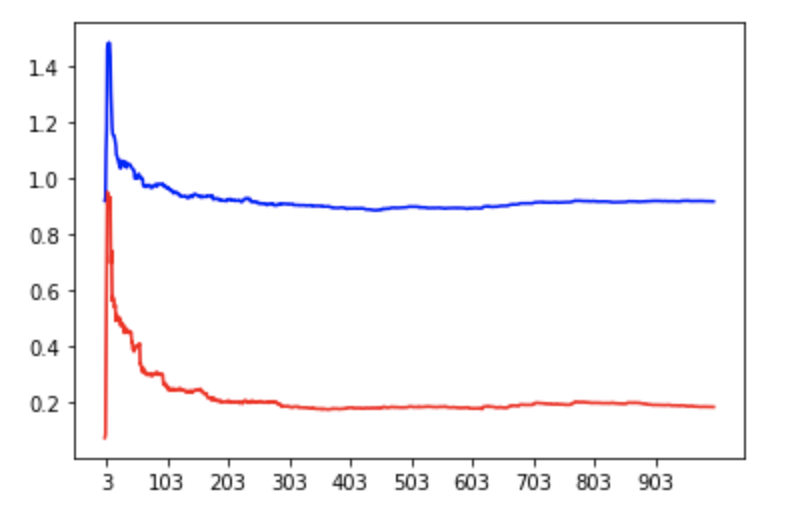
\includegraphics[width=.6\textwidth]{imagens/utilizacao2.png}
    \caption{Métricas \(\times\) Eventos Tratados --
        utilização de 0.2}
\end{figure}

\begin{figure}[h!]
    \centering
    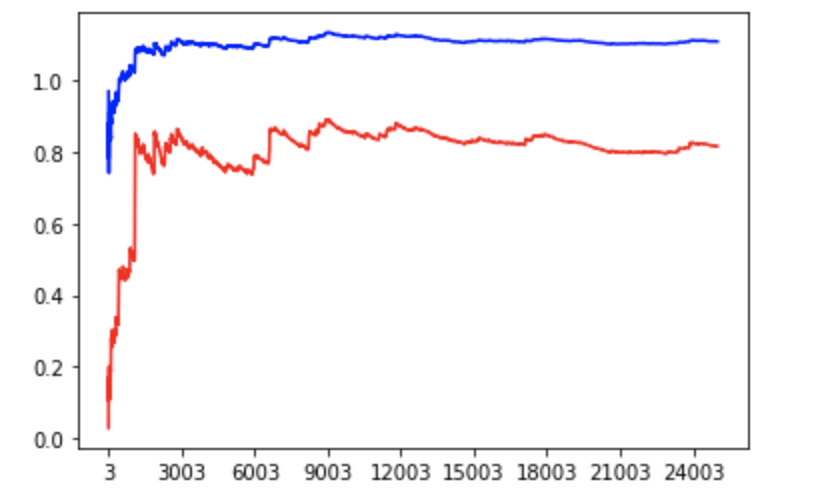
\includegraphics[width=.6\textwidth]{imagens/utilizacao4.png}
    \caption{Métricas \(\times\) Eventos Tratados --
        utilização de 0.4}
\end{figure}

\begin{figure}[h!]
    \centering
    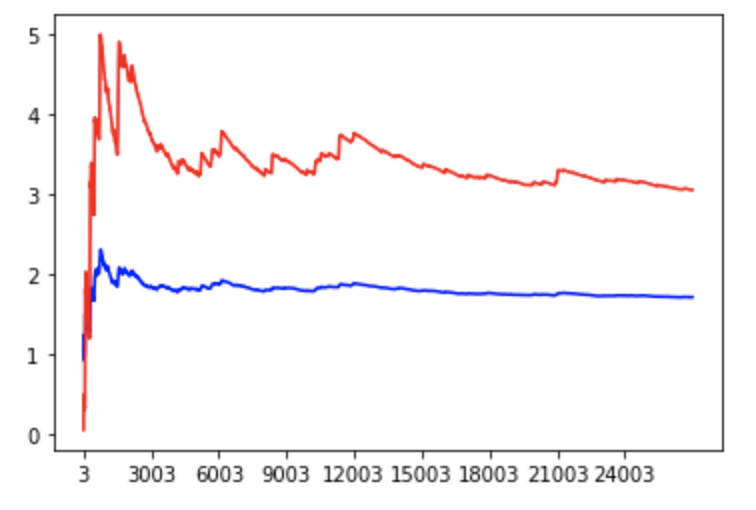
\includegraphics[width=.6\textwidth]{imagens/utilizacao6.png}
    \caption{Métricas \(\times\) Eventos Tratados --
        utilização de 0.6}
\end{figure}

\begin{figure}[h!]
    \centering
    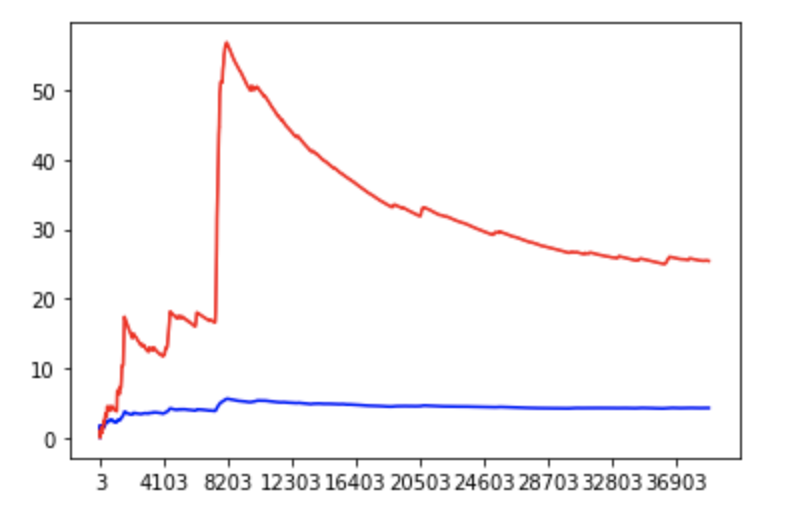
\includegraphics[width=.6\textwidth]{imagens/utilizacao8.png}
    \caption{Métricas \(\times\) Eventos Tratados --
        utilização de 0.8}
\end{figure}

\begin{figure}[h!]
    \centering
    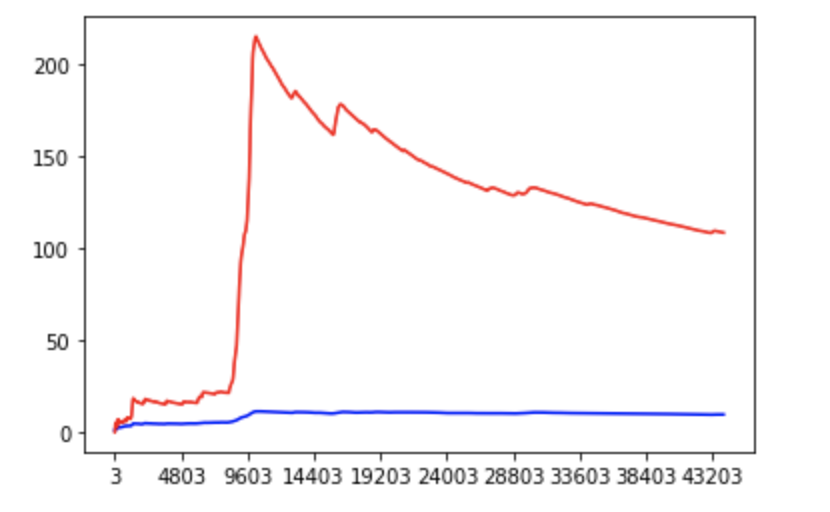
\includegraphics[width=.6\textwidth]{imagens/utilizacao9.png}
    \caption{Métricas \(\times\) Eventos Tratados --
        utilização de 0.9}
\end{figure}

\newpage
\section{Dedução dos Valores Analíticos}
\subsection{Número médio de pessoas na fila}
Vamos analisar a evolução do número
deixado para trás na \(i\)-ésma e \((i+1)\)-ésima partidas.
Seja \(N_i\) e  \(N_{i+1}\) os números de pessoas
deixadas para trás nestes instantes rescpectivamente.
Seja \(K\) o número de chegadas Poisson
durante um serviço \(X\),
com \(K(z) = X^*(\lambda - \lambda \; z)\).

Para uma fila M/M/1 \(\rho = \lambda \; \E{X}\)
\begin{align*}
    K'(1) &= -\lambda \; {X^*}'(0) = \lambda \; \E{X}
        = \rho \\
    K''(1) &= \lambda^2 \; {X^*}''(0)
        = \lambda^2 \; \E{X^2} = 2 \; \rho^2 \\
    K'''(1) &= - \lambda^3 \; {X^*}'''(0)
        = \lambda^3 \; \E{X^3} = 6 \; \rho^3
\end{align*}
Desse modo:
\[
    N_{i+1} = \begin{cases}
        K           \quad&, \qquad\text{se } N = 0 \\
        N_i + K - 1 \quad&, \qquad\text{se } N > 0 \\
    \end{cases}
\]
Usando tranformadas e condicionamentos, temos:
\[
    \E{z^{N_{i+1}}}
        = \E{z^{K} | N_i = 0} \; P(N_i = 0)
        + \E{z^{N_{i}+K-1} | N_i > 0} \; P(N_i > 0)
\]
No comportamento limite
\(N_i \Rightarrow N\) e \(N_{i+1} \Rightarrow N\)
com \(i \Rightarrow \infty\),
e para \(\rho < 1 \),
haverá uma distribuição estacionária
do número de pessoas na fila com T.~Z dada por
\(N(z) = \E{z^N}\).
Assim sendo, temos:
\begin{align*}
    \E{z^N} &= \E{z^K | N = 0} \; P(N = 0)
        + \E{z^{N+K-1} | N>0} \; P(N > 0) \\
    &= K(z) \; (1 - \rho)
        + \frac{K(z)}{z} \E{z^N | N > 0} \; \rho
\end{align*}
Entretando, sabemos que:
\begin{align*}
    \E{z^N} &= \E{z^N| N = 0} \; P(N = 0)
        + \E{z^N  | N > 0} \; P(N > 0) \\
    N(z) &= (1 - \rho) + \E{z^N | N > 0} \rho \\
    \E{z^N | N > 0} &= \frac{N(z) - (1 - \rho)}{\rho}
\end{align*}
Substituindo \(\E{z^N | N > 0}\)
na expressão anterior obtemos:
\begin{align*}
    N(z) &= K(z) \; (1 - \rho)
        + \frac{K(z)}{z} \; \frac{N(z) - (1 - \rho)}{\rho}
        \; \rho \\
    N(z) &= \frac{z \; K(z) \; (1 - \rho)
        + K(z) \; N(z) - K(z) \; (1 - \rho)}{z} \\
    z \; N(z) &= z \; K(z) \; (1 - \rho)
        + K(z) \; N(z) - K(z) \; (1 - \rho) \\
    N(z) \; (z - K(z)) &= K(z) \; (1 - \rho) \; (z - 1) \\
    N(z) &= \frac{K(z) \; (1 - \rho) \; (1 - z)}{K(z) - z}
\end{align*}
A partir de N(z),
podemos obter a \(\E{N}\),
uma vez que \(\E{N} = N'(1)\).
Derivando \(N(z)\) pela primeira vez:
\begin{align*}
    N(z) \; (K(z) - z) &= K(z) \; (1 - \rho) \; (1-z) \\
    N'(z) \; (K(z) - z) +  N(z) \; (K'(z) - 1)
        &= (1 - \rho) \; (K'(z) \; (1 - z) - K(z))
\end{align*}
Derivando novamente para retirar as indeterminações:
\begin{align*}
    N''(z) \; (K(z) - z) + N'(z) \; (K'(z) - 1)
        + N'(z) \; (K'(z) - 1) \\
        + N(z) \; (K''(z)) \\
    = (1 - \rho) \; (K''(z) \; (1 - z) - K(z) - K(z))
\end{align*}
\[
   N''(z) \; (K(z) - z) + 2 \; N'(z) \; (K'(z) - 1)
        + N(z) \; (K''(z))
\] \[
    \qquad\qquad \quad
    = (1 - \rho) \; (K''(z) \; (1 - z) - 2 \; K(z))
\]
Fazendo \(z = 1\):
\begin{align*}
    N''(1) \; (K(1) - 1) + 2 \; N'(1) \; (K'(1) - 1)
        + N(1) \; K''(1) \\
        = (1 - \rho) \; (K''(1) \; (1 - 1) - 2 \; K(1))
\end{align*} \begin{align*}
    2 \; N'(1) \; (\lambda \; \E{X} - 1)
        + \lambda^2 \; \E{X^2}
        &= (1 - \rho)(- 2 \; \lambda \; \E{X}) \\
    N'(1) &= \frac{(1 - \rho) \; (2 \; \lambda \; \E{X})
        + \lambda^2 \; \E{X^2}}{1 - \lambda \; \E{X}}
\end{align*}
Para M/M/1:
\[
    N'(1) = \frac{(1 - \rho) \; 2 \; \rho
        + 2 \; \rho^2}{1 - \rho} \\
        = \frac{\rho}{1 - \rho}
\]
Com \(N(z)\) calculada, é fácil achar
o número de pessoas na fila de espera,
uma vez que:
\[
    N_q = \begin{cases}
        0       \quad&, \qquad\text{se } N = 0 \\
        N - 1   \quad&, \qquad\text{se } N > 0 \\
    \end{cases}
\]
\begin{align*}
    \E{z^{N_q}} &= \E{z^N| N = 0} \; P(N = 0)
        + \E{z^{N-1} | N > 0} \;P(N > 0) \\
    N_q(z) &= (1 - \rho) + \frac{N(z) - (1 - \rho)}{z \; \rho}
        \; \rho \\
    N_q(z) &= \frac{z \; (1 - \rho) + N(z) - (1 - \rho)}{z} \\
    N_q(z) &= \frac{N(z) - (1 - \rho) \; (1 - z)}{z} \\
\end{align*}
Derivando \(N_q(z)\) uma vez para calcular o primeiro momento
\(\E{N_q} = N_q'(1)\):
\begin{align*}
    N_q(z) \; z &= N(z) - (1 - \rho) \; (1 - z) \\
    N_q'(z) \; z + N_q(z) &= N'(z) + (1 - \rho)
\end{align*}
Fazendo \(z = 1\):
\begin{align*}
    N_q'(1) + N_q(1) &= N'(1) + (1 - \rho) \\
    N_q'(1) &= N'(1) - \rho \\
    &= \frac{\rho}{1 - \rho} - \rho \\
    &= \frac{\rho^2}{1 - \rho}
\end{align*}

\subsection{Variância do número de pessoas na fila}
Para achar a variância do número de pessoas na fila,
precisamos encontrar o segundo momento de \(N_q\),
que pode ser dados por \(E[N_q^2] = N_q'(1) + N_q''(1)\),
então precisamos derivar \(N_q(z)\) novamente.
\[
    N_q''(z) \; z + N_q'(z) + N_q'(z) = N''(z)
\]
Fazendo \(z = 1\):
\begin{align*}
    N_q''(1) \; 1 + N_q'(1) \; + N_q'(1) &= N''(1) \\
    N_q''(1) &= N''(1) - 2 \; N_q'(1)
\end{align*}
Logo,
\begin{align*}
    \E{N_q^2} &= N'(1) - \rho + N''(1) - 2 \; N_q'(1) \\
    \E{N_q^2} &= N'(1) - \rho + N''(1) - 2 \; (N'(1) - \rho) \\
    \E{N_q^2} &= \E{N^2} - 2 \; \E{N} + \rho
\end{align*}
Como já temos o primeiro momento \(\E{N}\) calculado,
precisamos agora achar o segundo momento \(\E{N^2}\).
Derivando \(N(z)\) pela terceira vez vamos obter:
\begin{align*}
    N'''(z) \; (K(z) - z) + N''(z) \; (K'(z) - 1)
        + 2 \; N''(z) \; (K'(z) - 1) \\
        + 2 \; N'(z) \; (K''(z)) + N'(z) \; (K''(z))
        + N(z) \; (K'''(z)) \\
        = (1 - \rho) \; (-2 \; K''(z) - K''(z)
        + (1 - z) \; K'''(z))
\end{align*} \begin{align*}
    N'''(z) \; (K(z) - z) + 3 \; N''(z) \; (K'(z) - 1)
        + 3 \; N'(z) \; K''(z) \\
        + N(z) \; K'''(z)
        = (1 - \rho) \; (-3 \; K''(z) + (1 - z) \; K'''(z))
\end{align*}
Fazendo \(z = 1\):
\begin{align*}
    3 \; N''(1) \; (K'(1) - 1)
        + 3 \; N'(1) \; K''(1) + K'''(1)
        = (1 - \rho) \; (-3 \; K''(1))
\end{align*} \begin{align*}
    3 \; N''(1) \; (1 - \lambda \; \E{X})
        - 3 \; N'(1) \; (\lambda^2 \; \E{X^2})
        - \lambda^3 \; \E{X^3} \\
        = (1 - \rho) \; (3 \; \lambda^2 \; \E{X^2})
\end{align*} \begin{align*}
    3 \; N''(1) \; (1 - \lambda \; \E{X})
        = (1 - \rho) \; (3 \; \lambda^2 \; \E{X^2})
        + 3 \; N'(1) \; (\lambda^2 \; \E{X^2}) \\
        + \lambda^3 \; \E{X^3}
\end{align*} \begin{align*}
    3 \; N''(1) \; (1 - \lambda \; \E{X})
        = (1 - \rho) \; (3 \; \lambda^2 \; \E{X^2}) \\
        + \frac{3 \; (\lambda^2 \; \E{X^2}) \;
            ((1 - \rho) \; (2 \; \lambda \; \E{X})
        + \lambda^2 \; \E{X^2})}{2 \; (1 - \lambda \; \E{X})}
        &+ \lambda^3 \; \E{X^3} \\
\end{align*} \begin{align*}
    3 \; N''(1) \; (1 - \lambda \E{X})
        = \biggl[
            6 \; (1 - \rho) \; (\lambda^2 \; \E{X^2})
                \; (1 - \lambda \; \E{X}) \\
            + 3 \; (\lambda^2 \; \E{X^2}) \; ((1 - \rho)
                \; (2 \; \lambda \; \E{X}) + \lambda^2 \; \E{X^2}) \\
            + 2 \; (1 - \lambda \; \E{X}) \; (\lambda^3 \; \E{X^3})
        \biggr]
        \; \frac{1}{2 \; (1 - \lambda \; \E{X})}
\end{align*} \begin{align*}
    N''(1) = \biggl[
        6 \; (1 - \rho) \; (\lambda^2 \; \E{X^2})
            \; (1 - \lambda \; \E{X}) \\
        + 3 \; (\lambda^2 \; \E{X^2})
            \; ((1 - \rho) \; (2 \; \lambda \; \E{X})
        + \lambda^2 \; \E{X^2}) \\
        + 2 \; (1 - \lambda \; \E{X}) \; \lambda^3 \; \E{X^3}
    \biggr]
    \; \frac{1}{6 \; (1 - \lambda \; \E{X})^2}
\end{align*}
Logo \(\E{N^2} = N''(1) + N'(1)\)
para uma fila M/M/1, pode ser dado por:
\begin{align*}
    \biggl[
        12 \; (1 - \rho)^2 \; \rho^2
        + 6 \; \rho^2 \; ((1 - \rho) \; 2 \; \rho
        + 2 \; \rho^2) + 12 \; (1 - \rho) \; \rho^3 \\
        + 3 \; (1 - \rho) \; (2 \; \rho (1 - \rho)
        + 2 \; \rho^2)
    \biggr] \; \frac{1}{6 \; (1 - \rho)^2}
\end{align*} \begin{align*}
    \biggl[
        6 \; \rho - 6 \; \rho^2 + 12 \; \rho^2
        - 24 \; \rho^3 + 12 \; \rho^4 + 12 \; \rho^3
        + 12 \; \rho^3 - 12 \; \rho^4
    \biggr] \; \frac{1}{6 \; (1 - \rho)^2}
\end{align*} \begin{align*}
    \frac{6 \; \rho^2 + 6 \; \rho}{6 \; (1 - \rho)^2} \\
    \frac{\rho^2 + \rho}{(1 - \rho)^2}
\end{align*}
Agora podemos calcular \(E[N_q^{2}]\)
\begin{align*}
    \E{N_q^2} &= \frac{\rho^2 + \rho}{(1 - \rho)^2}
        - \frac{2 \; \rho}{(1 - \rho)} + \rho \\
    &= \frac{\rho^2 + \rho - 2 \;\rho + 2 \; \rho^2
        + \rho - 2 \; \rho^2 + \rho^3}{(1 - \rho)^2} \\
    &= \frac{\rho^2 + \rho^3}{(1 - \rho)^2}
\end{align*}
Por fim, calculamos a variância do número de pessoas
na fila de espera de uma M/M/1:
\begin{align*}
    V(N_q) &= \frac{\rho^2 + \rho^3}{(1 - \rho)^2}
        - (\frac{\rho^2}{1 - \rho})^2 \\
    &=\frac{\rho^2 + \rho^3 - \rho^4}{(1-\rho)^2}
\end{align*}

\subsection{Tempo médio em uma fila de espera FCFS}

Acompanhando um freguês tíıpico em uma fila M/G/1 FCFS,
podemos observar que o número deixado para trás é
exatamente o número de pessoas que chegou
durante o tempo \(T\) que o freguês típico passou no sistema.
Como o processo de chegada é Poisson
e relacionando as chegadas ao intervalo de tempo em
que as chegadas ocorreram,
pode-se escrever
\[
    N(z) = T(\lambda - \lambda \; z)
\]
Fazendo \(s = \lambda - \lambda \; z\)
e substituindo \(z = \frac{\lambda - s}{\lambda}\),
temos:
\[
    T^*(s) =
    \frac{(1 - \rho)\; s \; X^*(s)}{s - \lambda + \lambda \; X^*(s)}
\]
Sabemos que \(T = W + X\), como \(W\) e \(X\)
são independentes em uma fila FCFS,
então  \(T^*(s) =  W^*(s) \; X^*(s)\),
logo a transformada de Laplace
da pdf do tempo de espera na fila é dada por:
\[
    W^*(s) = \frac{(1 - \rho) \; s}{s - \lambda + \lambda \; X^*(s)}
\]
O tempo médio de espera na fila
pode ser facilmente obtido derivando \(W^{*}(s)\),
uma vez que \(E[W] = - W^{*'}(0)\).
Dessa forma, derivando em relação a \(s\) temos:
\begin{align*}
    W^*(s)(s - \lambda + \lambda \; X^*(s)) &= (1 - \rho) \; s \\
    {W^*}'(s) \; (s - \lambda + \lambda \; X^*(s))
        + W^*(s) \; (1 + \lambda \; {X^*}'(s)) &= (1 - \rho)
\end{align*}
Derivando novamente para retirar a ideterminação:
\begin{align*}
    {W^*}''(s) \; (s - \lambda + \lambda \; X^*(s))
        + {W^*}'(s) \; (1 + \lambda \; {X^*}'(s)) \\
        + {W^*}'(s) \; (1 + \lambda \; {X^*}'(s))
        + W^*(s) \; (\lambda \; {X^*}''(s)) = 0
\end{align*}
Fazendo \(s = 0\)
\begin{align*}
    2 \; {W^*}'(0) \; (1 + \lambda \; {X^*}'(0))
        &= - \lambda \; {X^*}''(0) \\
    {W^*}'(0)
        &= \frac{-\lambda \; {X^*}''(0)}{1 + \lambda \; {X^*}'(0)} \\
    \E{W} &= \frac{\lambda \; \E{X^2}}{2 \; (1 - \lambda \; \E{X})}
\end{align*}
Como \(\E{X^2} = 2 \; \E{X} \; \E{Xr}\),
podemos escrever
\(
    \E{W} = \frac{\lambda \; 2 \; \E{X} \; \E{Xr}}{2
        \; (1 - \lambda \; \E{X})}
\).
Para a fila M/M/1,
como temos um serviço exponencial,
\(E[Xr] = E[X]\),
logo \(\E{W} = \frac{\rho \; \E{X}}{(1 - \rho)}\).
Para o nosso simulador o tempo médio de serviço é 1 segundo,
então
\[
    \E{W} = \frac{\rho}{(1 - \rho)}
\]

\subsection{Variância do tempo de espera em uma fila de espera FCFS}
Para o cálculo da variância
é preciso achar o segundo momento \(\E{W^2} = {W^*}''(0)\).
Assim sendo, derivando \(W^*(s)\) pela terceira vez:
\begin{align*}
    {W^*}''(s) \; (s - \lambda + \lambda \; X^*(s))
        + {W^*}'(s) \; (1 + \lambda \; {X^*}'(s))
        + {W^*}'(s) \; (1 + \lambda \; {X^*}'(s)) \\
        + W^*(s)(\lambda \; {X^*}''(s)) = 0 \\
\end{align*} \begin{align*}
    {W^*}'''(s) \; (s - \lambda + \lambda \; X^*(s))
        + {W^*}''(s) \; (1 + \lambda \; {X^*}'(s))
        + {W^*}''(s) \; (1 + \lambda \; {X^*}'(s)) \\
        + {W^*}'(s) \; (\lambda \; {X^*}''(s))
        + {W^*}''(s) \; (1 + \lambda \; {X^*}'(s))
        + {W^*}'(s) \; (\lambda \; {X^*}''(s)) \\
        + {W^*}'(s) \; (\lambda \; {X^*}''(s))
        + W^*(s) \; (\lambda \; {X^*}'''(s)) = 0
\end{align*}
Fazendo \(s = 0\):
\[
    3 \; {W^*}''(0) \; (1 + \lambda {X^*}''(s))
        + 3 {W^*}'(0) \; (\lambda \; {X^*}''(0))
        + \lambda \; {X^*}'''(0) = 0
\]
\begin{align*}
    3 \; {W^*}''(0) \; (1 - \lambda \; {X^*}''(s))
        &= -3 \; {W^*}'(0) \; (\lambda \; {X^*}''(0))
        - \lambda {X^*}'''(0) \\
    3 \; {W^*}''(0) \; (1 - \lambda \E{X^2})
        &= 3 \; \E{W} \; (\lambda \; \E{X^2})
        + \lambda \; \E{X^3} \\
    {W^*}''(0) &= \frac{3 \; \lambda \; \E{X^2}
        \; \lambda \; \E{X^2}}{6 \; (1 - \lambda \; \E{X^2})^2}
        + \frac{\lambda \; \E{X^3}}{3
        \; (1 - \lambda \; \E{X^2})} \\
    {W^*}''(0) &= \frac{\lambda \; \E{X^2} \; \lambda
        \; \E{X^2}}{2 \; (1 - \lambda \; \E{X^2})^2}
        + \frac{\lambda \; \E{X^3}}{3
        \; (1 - \lambda \; \E{X^2})} \\
    {W^*}''(0) &= 2 \; \E{W}^2
        + \frac{\lambda \; \E{X^3}}{3
        \; (1 - \lambda \; \E{X^2})} \\
    {W^*}''(0) &= E[W^2]
\end{align*}
Logo, para a fila M/M/1
\[
    \E{W^2}
    = 2 \; \E{W}^2 + \frac{\lambda \; \E{X^3}}{3 \; (1 - \rho)}
\]
Finalmente, podemos achar a variância para uma fila M/M/1 FCFS:
\begin{align*}
    V(W_{FCFS}) &= \E{W^2} - \E{W}^2 \\
    &= 2 \; \E{W}^2 + \frac{\lambda \; \E{X^3}}{3 \; (1 - \rho)}
        - \E{W}^2 \\
    &= \E{W}^2 + \frac{\lambda \; \E{X^3}}{3 \; (1 - \rho)} \\
    &= \frac{\lambda^2 \; \E{X^2}^2}{4 \; (1 - \rho)^2}
        + \frac{\lambda \; \E{X^3}}{3 \; (1 - \rho)} \\
    &= \frac{3 \; \lambda^2 \; \E{X^2}^2 + 4 \; \lambda \; \E{X^3}
        - 4 \; \rho \; \lambda \; \E{X^3}}{12 \; (1 - \rho)^2}
    \end{align*}
Como o tempo médio de serviço é 1 segundo, \(\lambda = \rho\)
\[
    V(W_{FCFS}) = \frac{3 \; \rho^2 \; \E{X^2}^2
        + 4 \; \rho \; \E{X^3} - 4 \; \rho^2 \; \E{X^3}}{12
        \; (1 - \rho)^2}
\]
O segundo e o terceiro momentos de uma exponencial,
com \(\mu = 1\) podem ser dados por:
\begin{align*}
    \E{X^2}
        &= \int_{0}^{\infty} \mu \; x^2 \; e^{-\mu x} \; dx
        = \frac{2}{\mu^2} = 2 \\
    \E{X^3}
        &= \int_{0}^{\infty} \mu \; x^3 \; e^{-\mu x} \; dx
        = \frac{6}{\mu^3} = 6
\end{align*}
Então,
\[
    V(W_{FCFS})
    = \frac{-12 \; \rho^2 + 24 \; \rho}{12 \; (1 - \rho)^2} = \frac{-\rho^2 + 2 \; \rho}{(1 - \rho)^2}
\]
\subsection{Tempo médio em uma fila de espera LCFS}
Quando um freguêes típico chega à fila, o instante de chegada
é equivalente a uma amostragem aleatória no tempo (PASTA)
e a fila  é encontrada com seus valores médios no tempo,
tanto na fila de espera quanto no serviço.
O serviço médio pendente neste instante  é dado
por \(\E{U_0} = \E{N_q}\;\E{X} + \E{N_s}\;\E{Xr}\), com \(\E{N_q} = \lambda\;\E{W}\).

Deste serviço pendente, a parte \(\E{W_0} = \E{N_s}\;\E{Xr} = \rho\;\E{Xr}\)
será executada antes da entrada do freguês típico em serviço.
Caso novas chegadas nãpo ocorressem após a chegada
do freguês típico, o tempo médio de espera seria dado simplesmente
pelo atraso \(\E{W_0}\). A expressão para \(\E{W_0}\) pode ser também
obtida condicionando no estado ocupado ou ocioso
encontrado ao chegar:
\[
    \E{W_0} = \E{W_0|ocupado} \; P(ocupado) + \E{W_0|ociso} \; P(ocioso) = \rho\;\E{Xr}
\]
Se a fila é encontrada ociosa o atraso até entrada em serviço é zero e se o servidor
está ocupado o serviço residual é o atraso mínimo a ser observado.
Entretanto, toda nova chegada que ocorre enquanto o fregues típico
ainda está na fila deespera será servida antes do freguês típico.
O tempo médio de espera na fila pode ser visto
como um período ocupado diferenciado iniciado por \(\E{W_0}\), logo:
\[
    \E{W_{LCFS}} = \frac{ \E{W_0}}{ 1-\rho} = \frac{ \rho\;\E{Xr}}{ 1-\rho},\;\rho < 1
\]
Como na fila M/M/1 \(\E{Xr} = \E{X}\), pela propriedade da falta de memória, e  \(\E{X} =1s\)
\(\E{W_LCFS}\) pode ser escrito como
\(\E{W_{LCFS}} = \frac{\rho}{1 - \rho}\), que
é o mesmo tempo médio de espera em uma fila FCFS, como esperado e discutido em aula.
\subsection{Variância do tempo de espera em uma fila LCFS}
Para calcular a variância do tempo de espera em uma fila LCFS, precisamos obter
a sua transfromada \(W_{LCFS}^*(s)\), que pode ser obtida diretamente da T.L
do período ocupado, condicionando no estado ocupado ou ocioso que a fila  é encontrada pelo freguês tépico.
Quando o sistema é encontrado ocupado, o serviço inicial do período ocupado  é dado pela vida residual do
serviço, que no caso da fila M/M/1 é o proprio serviço.
Assim, \(W_{LCFS}^*(s)\) é dado por:
\begin{align*}
    \E{e^{s \; W_{LCFS}} \;|\; ocupado} \; P(ocupado)
        + \E{e^{s \; W_{LCFS}} \;|\; ocioso} \; P(ocioso) \\
    \rho \; X^*(s + \lambda - \lambda \; G^*(s)) + (1 - \rho) \\
    \rho \; G^*(s) + (1 - \rho)
\end{align*}
Derivando uma vez e fazendo s = 0 obetmos o primeiro momento:
\[
    {W_{LCFS}^*}'(0)
        = \rho \; {G^*}'(0) = \frac{\rho \; \E{X}}{1 - \rho}
\]
Como esperado e visto anteriormente. Agora derivamos novamente, para achar o segundo momento:
\[
    {W_{LCFS}^*}''(0)
        = \rho \; {G^*}''(0)
        = \frac{\rho \; \E{X^2}}{(1 - \rho)^3}
\]
Para achar a variância:
\begin{align*}
    V(W_{LCFS}) &=
        \frac{\rho \; \E{X^2}}{(1 - \rho)^3}
        - \left( \frac{\rho \; \E{X}}{1-\rho} \right)^2 \\
    &= \frac{2 \; \rho}{(1 - \rho)^3}
        - \left( \frac{\rho}{1 - \rho} \right)^2 \\
    &= \frac{2 \; \rho - \rho^2 + \rho^3}{(1 - \rho)^3}
\end{align*}

Ao final obtivemos os seguintes valores analíticos:
\begin{table}[h]
    \centering
    \begin{tabular}{|c|cc|}\hline
        Variável & Média & Variância \\\hline
        $ W_{LCFS} $&$ \frac{\rho}{1-\rho} $&$
            \frac{2 \; \rho - \rho^2 + \rho^3}{(1-\rho)^3} $\\&&\\
        $ W_{FCFS} $&$ \frac{\rho}{1-\rho} $&$
            \frac{2 \; \rho - \rho^2}{(1 - \rho)^2} $\\&&\\
        $ N_q      $&$ \frac{\rho^2}{1 - \rho} $&$
            \frac{\rho^2 + \rho^3 - \rho^4}{(1 - \rho)^2} $\\\hline
    \end{tabular}
    \caption{Valores analíticos}
\end{table}

\newpage
\section{Tabelas com Resultados}
Todos os valores foram calculados usando 3200 rodadas.

\subsection{Fila FCFS}
\begin{table}[h!]
    \centering
    \begin{tabular}{|c|c|c|lr|c|c|}\hline
        \multirow{2}{4.35em}{Utilização}
            & \multirow{2}{3.95em}{Analítico}
            & \multirow{2}{4.4em}{Simulação}
            & \multicolumn{2}{|c|}{IC t-Student}
            & \multirow{2}{2.4em}{Kmin}
            & \multirow{2}{3.75em}{Rodadas} \\
        &&& Inf & Sup &&\\\hline
        $ 0.2 $&$ 0.25 $&$ 0.250578 $&$ 0.249339 $&$ 0.251817 $&$
            1100 $&$ 3200 $\\\hline
        $ 0.4 $&$ 0.66667 $&$ 0.664532 $&$ 0.660929 $&$ 0.668136 $&$
            1000 $&$ 3200 $\\\hline
        $ 0.6 $&$ 1.5 $&$ 1.496058 $&$ 1.489644 $&$ 1.502472 $&$
            3200 $&$ 3200 $\\\hline
        $ 0.8 $&$ 4 $&$ 4.011640 $&$ 3.988097 $&$ 4.035183 $&$
            4000 $&$ 3200 $\\\hline
        $ 0.9 $&$ 9 $&$ 8.936891 $&$ 8.869972 $&$ 9.072329 $&$
            4300 $&$ 3200 $\\\hline
    \end{tabular}
    \caption{Média do tempo de espera (FCFS)}
\end{table}

\begin{table}[h!]
    \centering
    \begin{tabular}{|c|c|c|lr|c|c|}\hline
        \multirow{2}{4.35em}{Utilização}
            & \multirow{2}{3.95em}{Analítico}
            & \multirow{2}{4.4em}{Simulação}
            & \multicolumn{2}{|c|}{IC t-Student}
            & \multirow{2}{2.4em}{Kmin}
            & \multirow{2}{3.75em}{Rodadas} \\
        &&& Inf & Sup &&\\\hline
        $ 0.2 $&$ 0.05 $&$ 0.050200 $&$ 0.049933 $&$ 0.050468 $&$
            1100 $&$ 3200 $\\\hline
        $ 0.4 $&$ 0.26667 $&$ 0.266992 $&$ 0.265455 $&$ 0.268529 $&$
            1000 $&$ 3200 $\\\hline
        $ 0.6 $&$ 0.9 $&$ 0.899492 $&$ 0.895337 $&$ 0.903646 $&$
            3200 $&$ 3200 $\\\hline
        $ 0.8 $&$ 3.2 $&$ 3.202387 $&$ 3.181935 $&$ 3.222838 $&$
            4000 $&$ 3200 $\\\hline
        $ 0.9 $&$ 8.1 $&$ 8.079803 $&$ 7.989058 $&$ 8.170548 $&$
            4300 $&$ 3200 $\\\hline
    \end{tabular}
    \caption{Média do número de clientes na fila de espera (FCFS)}
\end{table}

\begin{table}[h!]
    \centering
    \begin{tabular}{|c|c|lcr|c|c|}\hline
        \multirow{2}{4.35em}{Utilização}
            & \multirow{3}{3.95em}{Analítico}
            & \multicolumn{3}{|c|}{IC t-Student}
            & \multirow{3}{1em}{K}
            & \multirow{3}{3.75em}{Rodadas} \\
        && Inf & Centro & Sup &&\\
        && \multicolumn{3}{|c|}{IC Chi-Square} &&\\\hline
        \multirow{2}{2em}{0.2}
            &\multirow{2}{3em}{0.5625}
            &$ 0.554137 $&$ 0.559098 $&$ 0.564060 $
            &\multirow{2}{2em}{1200} & \multirow{2}{2em}{3200}\\
            &&$ 0.532680 $&$ 0.5601115 $&$ 0.587543 $&&\\\hline
        \multirow{2}{2em}{0.4}
            &\multirow{2}{3em}{1.7778}
            &$ 1.742943 $&$ 1.763068 $&$ 1.783193 $
            &\multirow{2}{2em}{1000} & \multirow{2}{2em}{3200}\\
            &&$ 1.679759 $&$ 1.7662615 $&$ 1.852764 $&&\\\hline
        \multirow{2}{2em}{0.6}
            &\multirow{2}{2em}{5.25}
            &$ 5.149998 $&$ 5.202697 $&$ 5.255396 $
            &\multirow{2}{2em}{3200} & \multirow{2}{2em}{3200}\\
            &&$ 4.956856 $&$ 5.21212  $&$ 5.467384 $&&\\\hline
        \multirow{2}{2em}{0.8}
            &\multirow{2}{2em}{24}
            &$ 23.509601 $&$ 23.935170 $&$ 24.360740 $
            &\multirow{2}{2em}{4300} & \multirow{2}{2em}{3200}\\
            &&$ 22.804172 $&$ 23.9785215 $&$ 25.152871 $&&\\\hline
        \multirow{2}{2em}{0.9}
            &\multirow{2}{2em}{99}
            &$ 95.433237 $&$ 97.497706 $&$ 99.562174 $
            &\multirow{2}{2.5em}{12000} & \multirow{2}{2em}{3200}\\
            &&$ 92.890687 $&$ 97.6742925 $&$ 102.457898 $&&\\\hline
    \end{tabular}
    \caption{Variância do tempo de espera (FCFS)}
\end{table}

\begin{table}[h!]
    \centering
    \begin{tabular}{|c|c|lcr|c|c|}\hline
        \multirow{2}{4.35em}{Utilização}
            & \multirow{3}{3.95em}{Analítico}
            & \multicolumn{3}{|c|}{IC t-Student}
            & \multirow{3}{1em}{K}
            & \multirow{3}{3.75em}{Rodadas} \\
        && Inf & Centro & Sup &&\\
        && \multicolumn{3}{|c|}{IC Chi-Square} &&\\\hline
        \multirow{2}{2em}{0.2}
            &\multirow{2}{3em}{0.0725}
            &$ 0.072231 $&$ 0.072800 $&$ 0.073370 $
            &\multirow{2}{2em}{1200} & \multirow{2}{2em}{3200}\\
            &&$ 0.069360 $&$ 0.072932 $&$ 0.076504 $&&\\\hline
        \multirow{2}{2em}{0.4}
            &\multirow{2}{3em}{0.55111}
            &$ 0.545911 $&$ 0.551984 $&$ 0.558057 $
            &\multirow{2}{2em}{1000} & \multirow{2}{2em}{3200}\\
            &&$ 0.525901 $&$ 0.5529835 $&$ 0.580066 $&&\\\hline
        \multirow{2}{2em}{0.6}
            &\multirow{2}{2em}{2.79}
            &$ 2.729260 $&$ 2.754135 $&$ 2.779009 $
            &\multirow{2}{2em}{3200} & \multirow{2}{2em}{3200}\\
            &&$ 2.623995 $&$ 2.759123 $&$ 2.894251 $&&\\\hline
        \multirow{2}{2em}{0.8}
            &\multirow{2}{2em}{18.56}
            &$ 18.079828 $&$ 18.387566 $&$ 18.695303 $
            &\multirow{2}{2em}{4300} & \multirow{2}{2em}{3200}\\
            &&$ 17.518706 $&$ 18.420869 $&$ 19.323032 $&&\\\hline
        \multirow{2}{2em}{0.9}
            &\multirow{2}{2em}{88.29}
            &$ 85.524726 $&$ 87.415661 $&$ 89.306595 $
            &\multirow{2}{2.5em}{12000} & \multirow{2}{2em}{3200}\\
            &&$ 83.285045 $&$ 87.5739875 $&$ 91.862929 $&&\\\hline
    \end{tabular}
    \caption{Variância do número de clientes
    na fila de espera (FCFS)}
\end{table}

\subsubsection{FCFS: Evoluções dos ICs}
\begin{itemize}
    \item Utilização 0.2
    \begin{table}[h!]
        \centering
        \begin{tabular}{|c|c|lcr|lcr|}\hline
            \multirow{2}{3.75em}{Rodadas}
                & \multirow{2}{1em}{K}
                & \multicolumn{3}{|c|}{IC t-Student}
                & \multicolumn{3}{|c|}{IC Chi-Square} \\
            && Inf & Centro & Sup & Inf & Centro & Sup \\\hline
            3200 & 1100
                &$ 0.549500 $&$ 0.554831 $&$ 0.560163 $
                &$ 0.528614 $&$ 0.555836 $&$ 0.583058 $\\\hline
            3200 & 1200
                &$ 0.554137 $&$ 0.559098 $&$ 0.564060 $
                &$ 0.532680 $&$ 0.5601115 $&$ 0.587543 $\\\hline
        \end{tabular}
        \caption{Evolução da variância do tempo de espera --
            utilização 0.2 (FCFS)}
    \end{table}
    \item Utilização 0.8
    \begin{table}[h!]
        \centering
        \begin{tabular}{|c|c|lcr|lcr|}\hline
            \multirow{2}{3.75em}{Rodadas}
                & \multirow{2}{1em}{K}
                & \multicolumn{3}{|c|}{IC t-Student}
                & \multicolumn{3}{|c|}{IC Chi-Square} \\
            && Inf & Centro & Sup & Inf & Centro & Sup \\\hline
            3200 & 4000
                &$ 22.723773 $&$ 23.086594 $&$ 23.449415 $
                &$ 21.995693 $&$ 23.1284085 $&$ 24.261124 $\\\hline
            3200 & 4100
                &$ 22.877519 $&$ 23.249955 $&$ 23.622390 $
                &$ 22.151334 $&$ 23.2920645 $&$ 24.432795 $\\\hline
            3200 & 4200
                &$ 22.847088 $&$ 23.206213 $&$ 23.565338 $
                &$ 22.109659 $&$ 23.2482435 $&$ 24.386828 $\\\hline
            3200 & 4300
                &$ 23.509601 $&$ 23.935170 $&$ 24.360740 $
                &$ 22.804172 $&$ 23.9785215 $&$ 25.152871 $\\\hline
        \end{tabular}
        \caption{Evolução da variância do tempo de espera --
            utilização 0.8 (FCFS)}
    \end{table}
    \item Utilização 0.9
    \begin{table}[h!]
        \centering
        \begin{tabular}{|c|c|lcr|lcr|}\hline
            \multirow{2}{3.75em}{Rodadas}
                & \multirow{2}{1em}{K}
                & \multicolumn{3}{|c|}{IC t-Student}
                & \multicolumn{3}{|c|}{IC Chi-Square} \\
            && Inf & Centro & Sup & Inf & Centro & Sup \\\hline
            3200 & 4300
                &$ 87.375983 $&$ 89.904690 $&$ 92.434497 $
                &$ 85.656462 $&$ 90.067525 $&$ 94.478588 $\\\hline
            3200 & 5300
                &$ 90.818652 $&$ 93.096839 $&$ 95.375025 $
                &$ 88.697773 $&$ 93.265455 $&$ 97.833137 $\\\hline
            3200 & 8300
                &$ 91.937129 $&$ 94.184284 $&$ 96.431438 $
                &$ 89.733833 $&$ 94.3548695 $&$ 98.975906 $\\\hline
            3200 & 10000
                &$ 93.840319 $&$ 95.888738 $&$ 97.937156 $
                &$ 91.357747 $&$ 96.0624105 $&$ 100.757074 $\\\hline
            3200 & 11000
                &$ 94.914793 $&$ 96.914955 $&$ 98.915116 $
                &$ 92.335473 $&$ 97.0904865 $&$ 101.845500 $\\\hline
            3200 & 12000
                &$ 95.433237 $&$ 97.497706 $&$ 99.562174 $
                &$ 92.890687 $&$ 97.6742925 $&$ 102.457898 $\\\hline
        \end{tabular}
        \caption{Evolução da variância do tempo de espera --
            utilização 0.9 (FCFS)}
    \end{table}
\end{itemize}

\subsection{Fila LCFS}
\begin{table}[h!]
    \centering
    \begin{tabular}{|c|c|c|lr|c|c|}\hline
        \multirow{2}{4.35em}{Utilização}
            & \multirow{2}{3.95em}{Analítico}
            & \multirow{2}{4.4em}{Simulação}
            & \multicolumn{2}{|c|}{IC t-Student}
            & \multirow{2}{2.4em}{Kmin}
            & \multirow{2}{3.75em}{Rodadas} \\
        &&& Inf & Sup &&\\\hline
        $ 0.2 $&$ 0.25 $&$ 0.250152 $&$ 0.248964 $&$ 0.251341 $&$
            1200 $&$ 3200 $\\\hline
        $ 0.4 $&$ 0.66667 $&$ 0.665933 $&$ 0.662841 $&$ 0.669025 $&$
            1400 $&$ 3200 $\\\hline
        $ 0.6 $&$ 1.5 $&$ 1.496743 $&$ 1.492677 $&$ 1.500808 $&$
            5900 $&$ 3200 $\\\hline
        $ 0.8 $&$ 4 $&$ 3.994512 $&$ 3.985804 $&$ 4.003220 $&$
            30000 $&$ 3200 $\\\hline
        $ 0.9 $&$ 9 $&$ 8.984672 $&$ 8.958928 $&$ 9.010416 $&$
            70000 $&$ 3200 $\\\hline
    \end{tabular}
    \caption{Média do tempo de espera (LCFS)}
\end{table}

\begin{table}[h!]
    \centering
    \begin{tabular}{|c|c|c|lr|c|c|}\hline
        \multirow{2}{4.35em}{Utilização}
            & \multirow{2}{3.95em}{Analítico}
            & \multirow{2}{4.4em}{Simulação}
            & \multicolumn{2}{|c|}{IC t-Student}
            & \multirow{2}{2.4em}{Kmin}
            & \multirow{2}{3.75em}{Rodadas} \\
        &&& Inf & Sup &&\\\hline
        $ 0.2 $&$ 0.05 $&$ 0.050158 $&$ 0.049902 $&$ 0.050414 $&$
            1200 $&$ 3200 $\\\hline
        $ 0.4 $&$ 0.26667 $&$ 0.267424 $&$ 0.266066 $&$ 0.268782 $&$
            1400 $&$ 3200 $\\\hline
        $ 0.6 $&$ 0.9 $&$ 0.899740 $&$ 0.897107 $&$ 0.902374 $&$
            5900 $&$ 3200 $\\\hline
        $ 0.8 $&$ 3.2 $&$ 3.198500 $&$ 3.191076 $&$ 3.205924 $&$
            30000 $&$ 3200 $\\\hline
        $ 0.9 $&$ 8.1 $&$ 8.105467 $&$ 8.082076 $&$ 8.128858 $&$
            70000 $&$ 3200 $\\\hline
    \end{tabular}
    \caption{Média do número de clientes na fila de espera (LCFS)}
\end{table}

\begin{table}[h!]
    \centering
    \begin{tabular}{|c|c|lcr|c|c|}\hline
        \multirow{2}{4.35em}{Utilização}
            & \multirow{3}{3.95em}{Analítico}
            & \multicolumn{3}{|c|}{IC t-Student}
            & \multirow{3}{1em}{K}
            & \multirow{3}{3.75em}{Rodadas} \\
        && Inf & Centro & Sup &&\\
        && \multicolumn{3}{|c|}{IC Chi-Square} &&\\\hline
        \multirow{2}{2em}{0.2}
            &\multirow{2}{3em}{0.71875}
            &$ 0.713348 $&$ 0.721617 $&$ 0.729887 $
            &\multirow{2}{2em}{1200} & \multirow{2}{2em}{3200}\\
            &&$ 0.687519 $&$ 0.722924 $&$ 0.758329 $&&\\\hline
        \multirow{2}{2em}{0.4}
            &\multirow{2}{3em}{3.25926}
            &$ 3.224278 $&$ 3.269136 $&$ 3.313993 $
            &\multirow{2}{2em}{1400} & \multirow{2}{2em}{3200}\\
            &&$ 3.114660 $&$ 3.2750565 $&$ 3.435453  $&&\\\hline
        \multirow{2}{2em}{0.6}
            &\multirow{2}{2em}{16.5}
            &$ 16.202029 $&$ 16.372836 $&$ 16.543643 $
            &\multirow{2}{2em}{5900} & \multirow{2}{2em}{3200}\\
            &&$ 15.599177 $&$ 16.40249  $&$ 17.205803 $&&\\\hline
        \multirow{2}{2em}{0.8}
            &\multirow{2}{2em}{184}
            &$ 181.632087 $&$ 183.429733 $&$ 185.227378 $
            &\multirow{2}{2em}{30000} & \multirow{2}{2em}{3200}\\
            &&$ 174.762205 $&$ 183.761959 $&$ 192.761713 $&&\\\hline
        \multirow{2}{2em}{0.9}
            &\multirow{2}{2em}{1719}
            &$ 1692.385319 $&$ 1713.164478 $&$ 1733.943637 $
            &\multirow{2}{2.5em}{70000} & \multirow{2}{2em}{3200}\\
            &&$ 1632.213038 $&$ 1716.26734 $&$ 1800.321657 $&&\\\hline
    \end{tabular}
    \caption{Variância do tempo de espera (LCFS)}
\end{table}

\begin{table}[h!]
    \centering
    \begin{tabular}{|c|c|lcr|c|c|}\hline
        \multirow{2}{4.35em}{Utilização}
            & \multirow{3}{3.95em}{Analítico}
            & \multicolumn{3}{|c|}{IC t-Student}
            & \multirow{3}{1em}{K}
            & \multirow{3}{3.75em}{Rodadas} \\
        && Inf & Centro & Sup &&\\
        && \multicolumn{3}{|c|}{IC Chi-Square} &&\\\hline
        \multirow{2}{2em}{0.2}
            &\multirow{2}{3em}{0.0725}
            &$ 0.072113 $&$ 0.072718 $&$ 0.073322 $
            &\multirow{2}{2em}{1200} & \multirow{2}{2em}{3200}\\
            &&$ 0.069282 $&$ 0.0728495 $&$ 0.076417 $&&\\\hline
        \multirow{2}{2em}{0.4}
            &\multirow{2}{3em}{0.55111}
            &$ 0.545040 $&$ 0.550439 $&$ 0.555837 $
            &\multirow{2}{2em}{1400} & \multirow{2}{2em}{3200}\\
            &&$ 0.524429 $&$ 0.5514355 $&$ 0.578442 $&&\\\hline
        \multirow{2}{2em}{0.6}
            &\multirow{2}{2em}{2.79}
            &$ 2.758380 $&$ 2.796462 $&$ 2.796462 $
            &\multirow{2}{2em}{5900} & \multirow{2}{2em}{3200}\\
            &&$ 2.646181 $&$ 2.7824515 $&$ 2.918722 $&&\\\hline
        \multirow{2}{2em}{0.8}
            &\multirow{2}{2em}{18.56}
            &$ 18.430844 $&$ 18.547782 $&$ 18.664721 $
            &\multirow{2}{2em}{30000} & \multirow{2}{2em}{3200}\\
            &&$ 17.671352 $&$ 18.581376 $&$ 19.491400 $&&\\\hline
        \multirow{2}{2em}{0.9}
            &\multirow{2}{2em}{88.29}
            &$ 87.298955 $&$ 88.040016 $&$ 88.781077 $
            &\multirow{2}{2.5em}{70000} & \multirow{2}{2em}{3200}\\
            &&$ 83.879898 $&$ 88.199473 $&$ 92.519048 $&&\\\hline
    \end{tabular}
    \caption{Variância do número de clientes
    na fila de espera (LCFS)}
\end{table}

\subsubsection{FCFS: Evoluções dos ICs}
\begin{itemize}
    \item Utilização 0.2
    \begin{table}[h!]
        \centering
        \begin{tabular}{|c|c|lcr|lcr|}\hline
            \multirow{2}{3.75em}{Rodadas}
                & \multirow{2}{1em}{K}
                & \multicolumn{3}{|c|}{IC t-Student}
                & \multicolumn{3}{|c|}{IC Chi-Square} \\
            && Inf & Centro & Sup & Inf & Centro & Sup \\\hline
            3200 & 1100
                &$ 0.549500 $&$ 0.554831 $&$ 0.560163 $
                &$ 0.528614 $&$ 0.555836 $&$ 0.583058 $\\\hline
            3200 & 1200
                &$ 0.554137 $&$ 0.559098 $&$ 0.564060 $
                &$ 0.532680 $&$ 0.5601115 $&$ 0.587543 $\\\hline
        \end{tabular}
        \caption{Evolução da variância do tempo de espera --
            utilização 0.2 (LCFS)}
    \end{table}
    \item Utilização 0.6
    \begin{table}[h!]
        \centering
        \begin{tabular}{|c|c|lcr|lcr|}\hline
            \multirow{2}{3.75em}{Rodadas}
                & \multirow{2}{1em}{K}
                & \multicolumn{3}{|c|}{IC t-Student}
                & \multicolumn{3}{|c|}{IC Chi-Square} \\
            && Inf & Centro & Sup & Inf & Centro & Sup \\\hline
            3200 & 4000
                &$ 22.723773 $&$ 23.086594 $&$ 23.449415 $
                &$ 21.995693 $&$ 23.1284085 $&$ 24.261124 $\\\hline
            3200 & 4100
                &$ 22.877519 $&$ 23.249955 $&$ 23.622390 $
                &$ 22.151334 $&$ 23.2920645 $&$ 24.432795 $\\\hline
        \end{tabular}
        \caption{Evolução da variância do tempo de espera --
            utilização 0.8 (LCFS)}
    \end{table}
\end{itemize}

\newpage
\section{Conclusão}
\subsection{Dificuldades}
Uma dificuldade encontrada foi achar o valor da distribuição
Chi-quadrado para as \(3200\) rodadas solicitadas, todas as
tabelas que pesquisamos na internet traziam a distribuição
para intervalos de confiaça com no máximo \(1000\) graus de
liberdade. Por fim descobrimos que a ferramenta R possui
a função \inlcode{qchisq()},
que nos retorna a distribuição da Chi-quadrado
para os critérios desejados.

\subsection{Otimizações}
Não foi feita nenhuma ``otimização'' própriamente dita.

\subsection{Melhorias}
\subsubsection{Fase Transiente}
Durante o cálculo da fase transiente,
rodamos o programa até 1000000 serem tratados
para pegarmos a média e variância do tempo da fila de espera.
Apenas isso é feito,
não reduzimos o tempo para uma estimativa.
Os tempos da fase transiente devem variar também de acordo
com a utilização,
como vimos na apostila e
observamos nos resultados apresentados nos gráficos da seção 3.
Inclusive, podemos observar que o sistema estabiliza
bem antes dos 1000000 eventos.
Todavia, tratamos a fase transiente da mesma forma
para todas utilizações.
O tempo total de simulação pode ter
uma redução considerável após essa mudança.

\subsubsection{Especialização da Lista de Eventos}
Outro a ser melhorado é a heap de eventos,
inicialmente criamos uma heap de mínimo
para armazenar e gerenciar os eventos da simulação,
entretanto com o passar da confecção do trabalho
percebemos que esta estrutura não era necessária uma vez que
durante a simulação da fila temos no máximo dois eventos
armazenados no sistema.
Então potencialmente seria mais rápido
a implementação de um buffer fixo e circular.

\subsection{Comentários}
A implementação do simulador e a análise de resultados foram
fatores que contribuiram para o aprendizado e entendimento
mais didático da disciplina,
conseguimos colocar em prática
o conhecimento teórico visto em sala de aula e construir
em grupo uma simulação orientada à eventos discretos.

\subsection{Erros Encontrados}
\begin{itemize}
    \item \textbf{Random Exponencial} \par
        Os testes de random exponencial falharam no sistema
        operacional do Windows.
    \item \textbf{Cálculo da variância} \par
        Ao relizamos os primeiros testes do nosso sistema,
        com base nos valores analíticos,
        percemos que o cáculo da variância,
        tanto para o tempo de espera na fila
        quanto para o número de pessoas na fila,
        estava sendo implementado de maneira incorreta.
        Foi positivo ter os valores analíticos
        como uma base comparativa de resultados da simulação,
        indicando possíveis erros de implementação.
\end{itemize}

\newpage
\section{Documentação do Programa}
O repositório do projeto se encontra em \par
\url{https://github.com/PolyTadeu/TrabFinalAD}

Para compilar o código é necessário apenas
um compilador de \lang{C}
e \inlcode{make} é um facilitador.
Partindo do diretório raíz do projeto,
a instrução para compilar usando \inlcode{make}:
\begin{verbatim}
    $ make
\end{verbatim}
Ou caso queira usar um compilador específico:
\begin{verbatim}
    $ CC=COMPILADOR make
\end{verbatim}
Caso não tenha \inlcode{make} instalado:
\begin{verbatim}
    $ COMPILADOR -Wall -Wextra -Werror -lm src/main -o main
\end{verbatim}
Onde nos dois últimos comandos,
\verb.COMPILADOR. deve ser substituído
pelo o compilador que deseja utilizar
(\inlcode{gcc} é um exemplo).

O executável (\inlcode{main}, por padrão)
pode receber flags adicionais para alterar valores padrão,
como: semente utilizada, tamanho da rodada,
taxa de chegada
(vai ser igual a utilização quando taxa de saída for 1),
entre outros.
Note que a ordem da especificação das flags não importa,
desde que o valor numérico siga imediatamente após
a flag especificada.
Para saber todas as flags e seus valores padrão
rode \inlcode{./main -{}-help}.
Um exemplo de execução para semente inicial \(40\),
tamanho da rodada \(150\) e utilização \(0.9\):
\begin{verbatim}
    $ ./main -k 150 --seed 40 --lambda 0.9
\end{verbatim}

\end{document}
